%%%%%%%%%%%%%%%%%%%%%%%%%%%%%%%%%%%%%%%%%%%%%%%%%%%%%%%%%%%%%%%%%%%%%%%%%%%%%%%%
%%
%%   BornAgain User Manual
%%
%%   homepage:   http://www.bornagainproject.org
%%
%%   copyright:  Forschungszentrum Jülich GmbH 2015
%%
%%   license:    Creative Commons CC-BY-SA
%%   
%%   authors:    Scientific Computing Group at MLZ Garching
%%               C. Durniak, M. Ganeva, G. Pospelov, W. Van Herck, J. Wuttke
%%
%%%%%%%%%%%%%%%%%%%%%%%%%%%%%%%%%%%%%%%%%%%%%%%%%%%%%%%%%%%%%%%%%%%%%%%%%%%%%%%%

\chapter{Small-angle scattering and the Born approximation}  \label{SSas}
\chaptermark{Small-angle scattering}

\index{Small-angle scattering|(}%

This chapter introduces the basic theory of small-angle scattering (SAS).
We specifically consider scalar neutron propagation,
adjourning the notationally more involved
vectorial theory of X-rays and polarized neutrons
to the later chapter~\ref{SPol}.
Our exposition is self-contained,
except for the initial passage from the microscopic
to the macroscopic Schrödinger equation,
which we outline only briefly (Sect.~\ref{Swave}).
The standard description of scattering in first order Born approximation
is introduced in a way that is suitable subsequent modification
into the distorted wave Born approximation
needed for grazing-incidence small-angle scattering (Sect.\ref{SBornApprox}).
Finally, we discuss how the physical scattering law
(the double differential cross section as function of the scattering vector~$\q$)
relates to the experimental detector image (Sect.\ref{SdetImg}).


%%%%%%%%%%%%%%%%%%%%%%%%%%%%%%%%%%%%%%%%%%%%%%%%%%%%%%%%%%%%%%%%%%%%%%%%%%%%%%%%
\section{Coherent neutron propagation}\label{Swave}
%%%%%%%%%%%%%%%%%%%%%%%%%%%%%%%%%%%%%%%%%%%%%%%%%%%%%%%%%%%%%%%%%%%%%%%%%%%%%%%%
\index{Wave propagation!neutrons|(}%
\index{Neutrons!wave propagation|(}%

\index{Schrodinger@Schrödinger equation!microscopic}%
The scalar wavefunction $\psi(\r,t)$
\nomenclature[2t020]{$t$}{Time}%
\nomenclature[2r040]{$\r$}{Position}%
\nomenclature[1ψ030 2r040 2t02]{$\psi(\r,t)$}{Microscopic neutron wavefunction}%
of a free neutron
is governed by the microscopic Schrödinger equation
\begin{equation}\label{ESchrodi}
  i\hbar\partial_t \psi(\r,t)
  = \left\{-\frac{\hbar^2}{2m}\Nabla^2+V(\r)\right\} \psi(\r,t).
\end{equation}
By assuming a time-independent potential $V(\r)$,
we have excluded inelastic scattering.
Therefore we only need to consider monochromatic waves
with given frequency~$\omega$.
\nomenclature[1ω 020]{$\omega$}{Frequency of incident radiation}%
In consequence, we have a stationary wavefunction
\begin{equation}\label{Estationarywave}
  \psi(\r,t) = \psi(\r)\e^{-i\omega t}.
\end{equation}
\nomenclature[1ψ030 2r040 0]{$\psi(\r)$}{Stationary wavefunction}%
The minus sign in the exponent of the phase factor
is an inevitable consequence of the standard form of the Schrödinger equation,
and is therefore called the \E{quantum-mechanical sign convention}.
It is also used in most optics textbooks.
\index{Wave propagation|seealso {Sign convention}}%
\index{Sign convention!wave propagation}%
\index{Conventions|see {Sign convention}}%
The opposite choice of a phase factor $\e^{+i\omega t}$ is 
called the \E{crystallographic sign convention},
and is used in much of the literature on X-ray scattering,
including some important texts on GISAXS (e.~g.\ \cite{ReLL09}).
Since we are concerned with both X-rays and neutrons,
we had to make a somewhat arbitrary choice:

\Note
{\indent In this manual, and in the program code of \BornAgain,
the quantum-mechanical sign convention~(\ref{Estationarywave}) is chosen.
This has implications for the sign of the imaginary part of the
refractive index,
\index{Index of refraction|see {Refractive index}}
\index{Refractive index!sign convention}%
as explained in Sect.~\ref{Sabsorption}.}

Inserting (\ref{Estationarywave}) in (\ref{ESchrodi}),
we obtain the stationary Schrödinger equation
\begin{equation}\label{EstatSchrodi}
  \left\{-\frac{\hbar^2}{2m}\Nabla^2+V(\r)-\hbar\omega\right\} \psi(\r) = 0.
\end{equation}
\nomenclature[2m020]{$m$}{Neutron mass}%
\nomenclature[2v130 2r040]{$V(\r)$}{Microscopic optical potential}%
\index{Potential|see {Optical potential}}%
\index{Optical potential!nuclear (microscopic)}%
The \E{nuclear} (or \E{microscopic})
\E{optical potential} $V(\r)$,
in a somewhat ``naive conception'' \cite[p.~7]{Sea89},
consists of a sum of delta functions,
representing Fermi's ``pseudopotential''.
\index{Fermi's pseudopotential}%
The superposition of the incident wave with the scattered waves
originating from each illuminated nucleus
results in \E{coherent forward scattering},
\index{Coherent forward scattering}%
in line with Huygens' principle.
\index{Huygens' principle}%

Coherent superposition also leads to \E{Bragg scattering}.
\index{Bragg scattering!by atomic lattices}%
However, Bragg scattering by atomic lattices only occurs at angles
far above the small-angle range covered in GISAS experiments.
Accordingly, it can be neglected in the analysis of GISAS data,
or at most, is taken into account as a loss channel.

Therefore,
we can neglect the atomic structure of $V(\r)$,
and perform some coarse graining to
arrive at a \E{continuum approximation}.
\index{Continuum approximation!neutron propagation}%
This is 
similar to the passage from
the microscopic to the macroscopic Maxwell equations.
The details are intricate \cite{Sea89,Lax51},
but the result \cite[eq.~2.8.32]{Sea89} looks very simple:
The macroscopic field equation
has still the form of a stationary Schrödinger equation,
\index{Schrodinger@Schrödinger equation!macroscopic}%
\begin{equation}\label{EmacrSchrodi}
  \left\{-\frac{\hbar^2}{2m}\Nabla^2+v(\r)-\hbar\omega\right\} \psi(\r) = 0,
\end{equation}
\nomenclature[1ψ030 2r040 2t020]{$\psi(\r,t)$}{Coherent wavefunction}%
\nomenclature[2v020 2r040]{$v(\r)$}{Macrosopic optical potential}%
where $\psi$ now stands for the \E{coherent wavefunction}
\index{Coherent wavefunction}%
\index{Wave propagation!coherent}%
obtained by superposition of
incident and forward scattered states,
and $v(\r)$ is the \E{macroscopic optical potential}.
\index{Optical potential!macroscopic}%
This potential is weak, and slowly varying compared to atomic length scales.
It can be rewritten in a number of ways,
especially in terms of a
\E{bound scattering length density}
\index{Scattering length density}%
$\rho_s(\r)$ \cite[eq.\ 2.8.37]{Sea89},
\nomenclature[1ρ 034 2s000 2r040]{$\rho_s(\r)$}{Scattering length density}%
\begin{equation}
  v(\r)=\frac{2\pi \hbar^2}{m}\rho_s(\r),  
\end{equation}
or of a \E{refractive index}~$n(\r)$
\nomenclature[2n020 2r040]{$n(\r)$}{Refractive index}%
\index{Refractive index} % !vs scattering length density}%
\index{Index of refraction|see {Refractive index}}%
defined by
\begin{equation}\label{EnRefrIndx}
  n(\r)^2\coloneqq 1-\frac{4\pi}{K^2}\rho_s(\r) = 1 -\frac{2m}{\hbar^2 K^2}v(\r).
\end{equation}
In the latter expression,
we introduced the \E{vacuum wavenumber}~$K$,
\nomenclature[2k120]{$K$}{Vacuum wavenumber, corresponding to the frequency~$\omega$}%
which is connected with the frequency~$\omega$ through the
\E{dispersion relation}
\begin{equation}
  \frac{\hbar^2 K^2}{2m} = \hbar\omega.
\end{equation}
Since we only consider stationary solutions~(\ref{Estationarywave}),
$\omega$ will not appear any further in our derivations.
Instead, we use~$K$ as the given parameter that characterizes the
incoming radiation.
In terms of $K$ and $n$,
the macroscopic Schrödinger equation (\ref{EmacrSchrodi})
can be rewritten as
\Emph{
\begin{equation}\label{EnSchrodi}
  \left\{\Nabla^2+K^2n(\r)^2\right\}\psi(\r) = 0.
\end{equation}\vspace*{-10pt}
}
This equation is the starting point for the analysis of all
small-angle scattering experiments,
whether under grazing incidence (GISAS) or not (regular SAS).
\index{SAS|see {Small-angle scattering}}%
\index{Small-angle scattering}%

\index{Wave propagation!neutrons|)}%
\index{Neutrons!wave propagation|)}%

%%%%%%%%%%%%%%%%%%%%%%%%%%%%%%%%%%%%%%%%%%%%%%%%%%%%%%%%%%%%%%%%%%%%%%%%%%%%%%%%
\section{Neutron scattering in Born approximation}\label{SBornApprox}
%%%%%%%%%%%%%%%%%%%%%%%%%%%%%%%%%%%%%%%%%%%%%%%%%%%%%%%%%%%%%%%%%%%%%%%%%%%%%%%%

%===============================================================================
\subsection{The Born expansion}\label{SBornExpans}
%===============================================================================

\index{Born approximation|(}%

To describe an elastic scattering experiment,
we need to solve the Schrödinger equation~(\ref{EnSchrodi})
under the asymptotic boundary condition
\begin{equation}\label{Escabouco}
  \psi(\r)
  \simeq \psi_\ti(\r) + f(\vartheta,\varphi)\frac{\e^{iKr}}{4\pi r}
  \text{~for~}r\to\infty,
\end{equation}
\nomenclature[1ψ034 2i000 2r040]{$\psi_\ti(\r)$}{Incident wavefunction}%
\nomenclature[2i000]{i}{Subscript ``incident''}%
where $\psi_\ti(\r)$ is the incident wave
as prepared by the experimental apparatus,
and the second term on the right-hand side is
the outgoing scattered wave
that carries information in form of the angular distribution
$f(\vartheta,\varphi)$.

For thermal or cold neutrons,
as for X-rays, the refractive index~$n$ is almost always
very close to~1.
This suggests a solution of the Schrödinger equation
by means of a perturbation expansion in powers of $n^2-1$.
This expansion is named after Max Born
who introduced it in quantum mechanics.\footnote
{It goes back to Lord Rayleigh
who devised it for sound,
and later also applied it to electromagnetic waves,
which resulted in his famous explanation of the blue sky.}

To carry out this idea, we rewrite the Schrödinger equation
once more so that it takes the form of a Helmholtz equation
\index{Helmholtz equation}%
with a perturbation term on the right side:
\begin{equation}\label{ESchrodiHelmholtz}
  \left(\Nabla^2+K^2\right)\psi(\r)
  = 4\pi\chi(\r)\psi(\r)
\end{equation}
with
\begin{equation}\label{EChiDef}
  \chi(\r) \coloneqq  \frac{K^2}{4\pi}\left(1-n^2(\r)\right).
\end{equation}
\nomenclature[1χ030 2r040]{$\chi(\r)$}{Perturbative potential, for neutrons equal to the scattering-length density~$\rho_s$}%
This definition just compensates (\ref{EnRefrIndx}) so that $\chi=\rho_s$.
In the following, we prefer the notation~$\chi$
and the appellation \E{perturbative potential}
\index{Potential|see {Perturbation}}%
\index{Perturbation}%
over the scattering length density~$\rho_s$
to prepare for the generalization to the electromagnetic case.

Equation~(\ref{ESchrodiHelmholtz}) looks
like an inhomogeneous differential equation ---
provided we neglect for a moment that the unknown function~$\psi$
reappears on the right side.
The homogeneous equation
\begin{equation}\label{EHelmholtzHomog}
  \left(\Nabla^2+K^2\right)\psi(\r) = 0
\end{equation}
is solved by plane waves and superpositions thereof.
It applies in particular to the incident wave~$\psi_\ti$.

For an isolated inhomogeneity,
\begin{equation}\label{EHelmholtzForGreen}
  \left(\Nabla^2+K^2\right)G(\r,\r') = \delta(\r-\r')
\end{equation}
\nomenclature[2g130 2r040 2r041]{$G(\r,\r')$}{Green function}%
\index{Green function!homogeneous material}%
is solved by the Green function\footnote
{Verification under the condition $\r\ne0$
is a straightforward exercise in vector analysis.
For the special case $\r=0$,
one encloses the origin in a small sphere
and integrates by means of the Gauss-Ostrogadsky divergence theorem.
This explains the appearance of the factor $4\pi$.}
\begin{equation}\label{EGreens1}
  G(\r,\r') = \frac{\e^{iK|\r-\r'|}}{4\pi |\r-\r'|},
\end{equation}
which is an outgoing spherical wave centered at $\r'$.
Convoluting this function with the given inhomogeneity $4\pi\chi\psi$,
we obtain what is known as the Lippmann-Schwinger equation,
\index{Lippmann-Schwinger equation}%the formal solution
\begin{equation}\label{EPsiFormal}
  \psi(\r)
  = \psi_\ti(\r)
  + \int\!\d^3r'\, G(\r,\r') 4\pi\chi(\r')\psi(\r').
\end{equation}
This integral equation for $\psi(\r)$ improves
upon the original stationary Schrödinger equation (\ref{ESchrodiHelmholtz})
in that it ensures the boundary condition~(\ref{Escabouco}).
It can be resolved into an infinite series
by iteratively substituting the full right-hand side of~(\ref{EPsiFormal})
into the integrand.
Successive terms in this series contain rising powers of $\chi$.
Since $\chi$ is assumed to be small, the series is likely to converge.
In \E{first-order Born approximation},
only the linear order in $\chi$ is retained,
\begin{equation}\label{EBorn}
  \psi(\r)
  \doteq \psi_\ti(\r)
  + 4\pi \int\!\d^3r'\, G(\r,\r') \chi(\r') \psi_\ti(\r').
\end{equation}
This is practically always adequate for
material investigations with X-rays or neutrons,
where the aim is to 
deduce $\chi(\r')$ from the scattered intensity ${|\psi(\r)|}^2$.
Since detectors are always placed at positions $\r$
that are not illuminated by the incident beam,
we are only interested in the scattered wave field
\begin{equation}\label{EBornS}
  \psi_\text{s}(\r)
  \coloneqq 
  4\pi \int\!\d^3r'\, G(\r,\r') \chi(\r') \psi_\ti(\r').
\end{equation}
\nomenclature[1ψ034 2s000 0 2r040]{$\psi_\text{s}(\r)$}{Scattered wavefunction}%
\nomenclature[2s000 0]{s}{Subscript ``scattered''}%

\index{Born approximation|)}%

%===============================================================================
\subsection{Far-field approximation}
%===============================================================================

\index{Far-field approximation|(}%

We can further simplify (\ref{EBornS})
under the conditions of Fraunhofer diffraction:
\index{Fraunhofer approximation}%
the distance from the sample to the detector location~$\r$
must be much larger than the size of the sample.
Since the scattered wave $\psi_\text{s}(\r)$
only depends on $\r$ through the Green function~$G(\r,\r')$,
we shall derive a far-field approximation for the latter.

We choose the origin within the sample
so that the integral in~(\ref{EBornS}) runs over $\r'$ with $r'\ll r$.
This allows us to expand
\begin{equation}
  \left|\r-\r'\right|
  \doteq \sqrt{r^2-2\r\,\r'}
  \doteq r - \frac{\r\,\r'}{r}
  \equiv r - \frac{\k_\tf \r'}{K},
\end{equation}
\nomenclature[2f000]{f}{Subscript ``final'', for outgoing waves scattered into the direction of the detector}%
\nomenclature[2k040]{$\k$}{wavevector}
where we have introduced the outgoing wavevector
\begin{equation}
  \k_\tf\coloneqq K\frac{\r}{r}.
\end{equation}
We apply this to~(\ref{EGreens1}),
\index{Green function!homogeneous material}%
and obtain in leading order the far-field Green function
\begin{equation}\label{EGreenFar}
  G_\text{far}(\r,\r')
  = \frac{\e^{iKr}}{4\pi r}\psi^*_\tf(\r')
\end{equation}
\nomenclature[2g134 2far]{$G_\text{far}(\r,\r')$}{Far-field approximation to the Green function $G(\r,\r')$}
where
\begin{equation}
  \psi_\tf(\r) \coloneqq  \e^{i\k_\tf \r}
\end{equation}
\nomenclature[1ψ034 2f000 2r040]{$\psi_\tf(\r)$}{Plane wave propagating from the sample towards the detector}%
is a plane wave propagating towards the detector,
and $\psi^*$ designates the complex conjugate of $\psi$.
With respect to $\r$, $G_\text{far}$ is an outgoing spherical wave.

The scattered wave~(\ref{EBornS})
becomes in the far-field approximation 
\begin{equation}\label{EsandwichC}
  \psi_\text{s,far}(\r)
  = \frac{\e^{iKr}}{r}
    \bra \psi_\tf|\chi|\psi_\ti\ket,
\end{equation}
\nomenclature[1ψ034 2s000 2far]{$\psi_\text{s,far}(\r)$}{Far-field approximation to the scattered wavefunction $\psi_\text{s}(\r)$}%
where we used Dirac notation for the transition matrix element
\index{Transition matrix}%
\begin{equation}\label{Etrama}
  \bra \psi_\tf|\chi|\psi_\ti\ket
  \coloneqq  \int\!\d^3r\, \psi^*_\tf(\r)\chi(\r)\psi_\ti(\r).
\end{equation}
\nomenclature[0$\langle$0]{{$\bra\ldots\vert\ldots\vert\ldots\ket$}}{Matrix element, defined as a volume integral}%
Making the standard assumption
that the incident radiation is a plane wave
\begin{equation}\label{EPsi0Plane}
  \psi_\ti(\r)=\e^{i \k_\ti \r}
\end{equation}
with $k_\ti=K$,
and introducing the \E{scattering vector}\footnote
{With this choice of sign,
\index{Sign convention!scattering vector}%
$\hbar\q$ is the momentum 
\index{Momentum transfer|see {Scattering vector}}%
\E{gained} by the scattered neutron,
and \E{lost} by the sample.
In much of the literature the opposite convention is prefered,
since it emphasizes the sample physics over the scattering experiment.
However, when working with twodimensional detectors
it is highly desirable to express pixel coordinates
\index{Coordinate system}
and scattering vector components 
with respect to equally oriented coordinate axes,
which can only be achieved by the convention~(\ref{Eq}).}
\index{Scattering vector}%
\begin{equation}\label{Eq}
  \q\coloneqq \k_\tf-\k_\ti,
\end{equation}
\nomenclature[2q040]{$\q$}{Scattering vector}%
we can rewrite (\ref{EsandwichC}) as
\begin{equation}\label{EBornBraChiKet}
  \bra \psi_\tf|\chi|\psi_\ti\ket
  = \int\!\d^3r\, \e^{-i\q\,\r}\chi(\r),
\end{equation}
which shows that neutron scattering,
in first-order Born approximation,
measures the Fourier transform
of the optical potential.
\index{Optical potential!Fourier transform}%
In order to save some minus signs later,
we take the complex conjugate of (\ref{EBornBraChiKet}) 
to define the abbreviation\footnote
{Physical results only depend on the squared modulus $|chi(\q)|^2$;
insofar the choice of sign is inconsequential.
\index{Sign convention!Fourier transform $\chi(\q)$}%
The choice~(\ref{EBornBraChiKet}) brings us back to conformity 
with the standard notation in the GISAXS literature,
like Eq.~(90) in \cite{ReLL09},
from which we deviated in (\ref{Estationarywave})
in order to preserve the standard form
of the Schrödinger equation~(\ref{ESchrodi}).}
\begin{equation}\label{EchiQdef}
   \chi(\q) \coloneqq \int\!\d^3r\, \e^{i\q\,\r}\chi(\r).
\end{equation}
\nomenclature[1χ030 2q040]{$\chi(\v{q})$}{Fourier transform of the perturbation potential $\chi(\r)$}%

\index{Far-field approximation|)}%


%===============================================================================
\subsection{Differential cross section}\label{SdiffCross}
%===============================================================================

In connection with (\ref{EBorn}) we mentioned
that a scattering experiment measures intensities~${|\psi(\r)|}^2$.
We shall now restate this in a more rigorous way.
In the case of neutron scattering,
one actually measures a \E{probability flux}.
We define it in arbitrary relative units as
\begin{equation}\label{EdefJ}
  \v{J}(\r) \coloneqq  \psi^*\frac{\Nabla}{2i}\psi - \psi\frac{\Nabla}{2i}\psi^*.
\end{equation}
\nomenclature[2j150 2r040]{$\v{J}(\r)$}{Probability flux}
\index{Flux!incident and scattered}%
The ratio of the scattered flux hitting an infinitesimal detector area
$r^2\d\Omega$ to the incident flux is expressed as a
\E{differential cross section}
\index{Cross section}%
\begin{equation}\label{Exsectiondef}
  \frac{\d\sigma}{\d\Omega}
  \coloneqq  \frac{r^2 J(\r)}{J_\ti}.
\end{equation}
\nomenclature[1ω120]{$\Omega$}{Solid angle}%
\nomenclature[1σ020]{$\sigma$}{Scattering or absorption cross section}%
The geometric factors that needed to
convert $\d\sigma/\d\Omega$ into detector counts shall be discussed
below in Sect.~\ref{SdetImg}.

With (\ref{EPsi0Plane}), the incident flux is
\begin{equation}\label{EJi}
  \v{J}_\ti = \k_\ti.
\end{equation}
With (\ref{EsandwichC}), the scattered flux at the detector is
\begin{equation}\label{EJr}
  \v{J}(\r)
  = \v{\hat r}\frac{K}{r^2}
    {\left|\bra\psi_\tf|\chi|\psi_\ti\ket\right|}^2.
\end{equation}
From (\ref{Exsectiondef}) we obtain 
the generic differential cross section of elastic scattering in first order Born approximation,
\Emph{
\begin{equation}\label{Exsection}
  \frac{\d\sigma}{\d\Omega}
  =  {\left|\bra\psi_\tf|\chi|\psi_\ti\ket\right|}^2.
\end{equation}\vspace*{-5pt}
}
As we shall see below,
it holds not only for plane waves governed
by the vacuum Helmholtz equation~(\ref{EHelmholtzHomog}),
but also for distorted waves.

In the plane-wave case considered here,
with the result (\ref{EBornBraChiKet}) and the abbreviation (\ref{EchiQdef}),
the differential cross section is just the squared modulus
of the Fourier transform 
\index{Scattering length density}%
of the scattering-length density.
\begin{equation}\label{Ecross1}
  \frac{\d\sigma}{\d\Omega}
  = {\left| \chi(\q) \right|}^2.
\end{equation}


%%%%%%%%%%%%%%%%%%%%%%%%%%%%%%%%%%%%%%%%%%%%%%%%%%%%%%%%%%%%%%%%%%%%%%%%%%%%%%%%
\section{Detector images}\label{SdetImg}
%%%%%%%%%%%%%%%%%%%%%%%%%%%%%%%%%%%%%%%%%%%%%%%%%%%%%%%%%%%%%%%%%%%%%%%%%%%%%%%%

\def\tc{\text{c}}

\begin{figure}[t]
\begin{center}
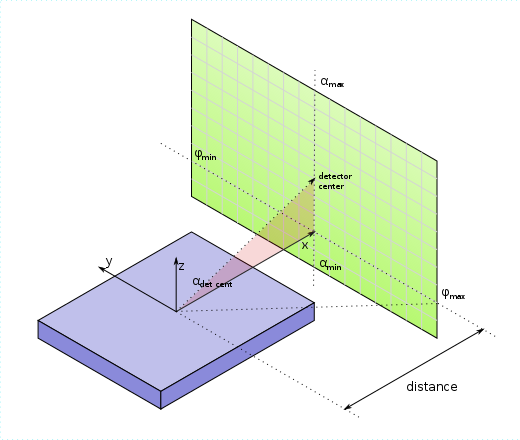
\includegraphics[width=.5\textwidth]{fig/drawing/experimental_geometry.png}
\end{center}
\caption{Experimental geometry with a twodimensional pixel detector.}
\label{FexpGeom}
\end{figure}

To conclude this chapter on the foundations of small-angle scattering,
we shall derive the geometric factors
that allow us to convert differential cross sections into detector counts.
We shall also discuss how to present data on a physically meaningful scale.

%===============================================================================
\subsection{Coordinate transform}
%===============================================================================

We assume that scattered radiation is detected in a flat,
two-dimensional detector
that generates histograms on a rectangular grid,
consisting of $n\cdot m$ pixels of constant width and height,
as sketched in Fig.~\ref{FexpGeom}.
This figure also shows the coordinate system
\index{Conventions|see {Coordinate system}}%
\index{Coordinate system}%
according to unanimous GISAS convention,
with $z$ normal to the sample plane,
and with the incident beam in the $xz$ plane.
The origin is at the sample position;
more precisely, it is for $x$ and $y$ at the center of the sample,
and for $z$ at the sample surface.
We suppose that the detector is mounted perpendicular to the $x$ axis
at a distance $L$ from the sample position.
%the $x$ axis intersects the detector plane at $(L,y_\tc,z_\tc)$.
The real-space coordinate at the center of pixel $(i,j)$ is $(L,y_i,z_i)$.
Each pixel has a width~$\Delta y$ and a height~$\Delta z$.
\index{Detector!pixel coordinate}%
\index{Pixel|see {Detector}}%

Since the differential scattering cross section (\ref{Exsectiondef})
is given with respect to a solid-angle element $\d\Omega$,
we need to express scattered wavevector $\k_\tf$ in spherical coordinates,
using the horizontal azimuth angle~$\phi_\tf$
and the vertical glancing angle $\alpha_\tf$.
The projection of $(\alpha_\tf,\phi_\tf)$ into
the detector plane~$(y,z)$ is known as the \E{gnomonic projection}.
\index{Gnomonic projection}%
\index{Projection!wave vector to pixel coordinate}%
From elementary trigonometry one finds
\begin{equation}\label{Eyzdet}
  \begin{array}{lcl}
  y &=& L \tan\phi_\tf,\\
  z &=& (L/ \cos\phi_\tf) \tan\alpha_\tf.
  \end{array}
\end{equation}
Fig.~\ref{Fconstalphi} shows lines of equal $\alpha_\tf$,~$\phi_\tf$
in the detector plane.

\begin{figure}[t]
\begin{center}
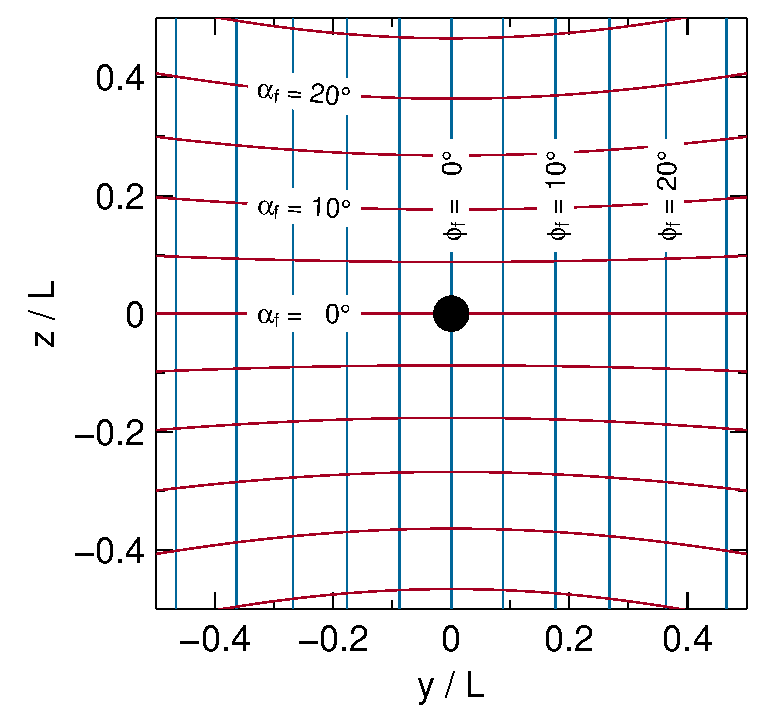
\includegraphics[width=.47\textwidth]{fig/drawing/SAS_const_alphi.ps}
\end{center}
\caption{Lines of constant $\alpha_\tf$ (red) or $\phi_\tf$ (blue)
in the detector plane,
for a planar detector at distance~$L$ from the sample.
The black dot indicates the beamstop location for 
the central incident beam ($\hat\k_\ti = \hat x$).}
\label{Fconstalphi}
\end{figure}

To determine the scattering vector $\q_{ij}$ 
that corresponds to a pixel $(i,j)$,
we need to express the outgoing wavevector~$\k_\tf$ as function of $y$ and~$z$.
This can be done either by inverting (\ref{Eyzdet})
and inserting the so obtained $\alpha_\tf(y,z)$ and $\phi_\tf(y)$ in
\begin{equation}\label{Ekf_by_angle}
  \k_\tf=K\left(\begin{array}{c}
   \cos\alpha_\tf\cos\phi_\tf\\
   \cos\alpha_\tf\sin\phi_\tf\\
   \sin\alpha_\tf\end{array}\right),
\end{equation}
or much more directly by using geometric similarity in Cartesian coordinates.
The result is rather simple:
\Emph{
\begin{equation}\label{Ekf_by_pixel}
  \k_\tf=\frac{K}{\sqrt{L^2+y^2+z^2}}\left(\begin{array}{c}
   L\\
   y\\
   z\end{array}\right).
\end{equation}
\vspace*{-5pt}}
The wavevector $\q_{ij}$ can then be determined through the following steps:
\begin{equation}\label{Eqalgo}
  \begin{array}{cl}
      (i,j)&\\
      \downarrow&\mbox{affine-linear relations}\\
      (y,z)\\
      \downarrow&\mbox{use (\protect\ref{Ekf_by_pixel})}\\
      \k_\tf&\\
      \downarrow&\mbox{use (\protect\ref{Eq})}\\
      \q&\\
  \end{array}
\end{equation}
where the first step is mathematically trivial,
but requires an experimental calibration of the origin of the $(x,y)$ scale.

The solid angle under which a detector pixel
is illuminated from the sample is in linear approximation
\begin{equation}
  \Delta\Omega
  = \cos\alpha_\tf\:\Delta\alpha_\tf\,\Delta\phi_\tf
  = \cos\alpha_\tf
    \left|\frac{\partial(\alpha_\tf,\phi_\tf)}{\partial(y,z)}\right|
    \Delta y \,\Delta z
  = \cos^3\!\alpha_\tf\, \cos^3\!\phi_\tf\: \frac{\Delta y \,\Delta z}{L^2}.
\end{equation}
\index{Detector!illumination angle correction factor}%
\index{Illumination!detector}%
Altogether,
the expected count rate in detector pixel $(i,j)$ is proportional to
\begin{equation}\label{EItrafo_cos}
  I_{ij} = \cos^3\!\alpha_\tf\, \cos^3\!\phi_\tf\:
          \frac{\partial\sigma}{\partial\Omega}(\q_{ij}),
\end{equation}
where we have omitted constant factors $L^{-2}$, $\Delta y$ and $\Delta z$.
Using pixel coordinates instead of angles, this can be rewritten as
\Emph{%
\begin{equation}\label{EItrafo_pix}
  I_{ij} = \left( 1+\frac{y^2+z^2}{L^2}\right)^{-3/2}
          \frac{\partial\sigma}{\partial\Omega}\bigl(\q_{ij}(y,z)\bigr).
\end{equation}
\vspace*{-2pt}}
%(usually as the centre between the transmitted
%and the specularly reflected beam spot).

%===============================================================================
\subsection{Data representation}
%===============================================================================

\begin{figure}[t]
\begin{center}
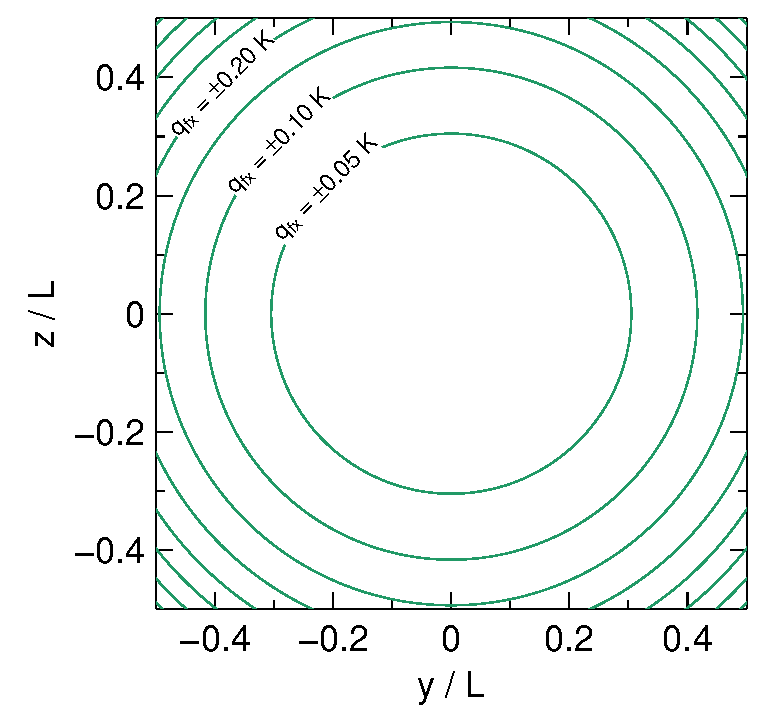
\includegraphics[width=.47\textwidth]{fig/drawing/SAS_const_q_x.ps}
\hfill
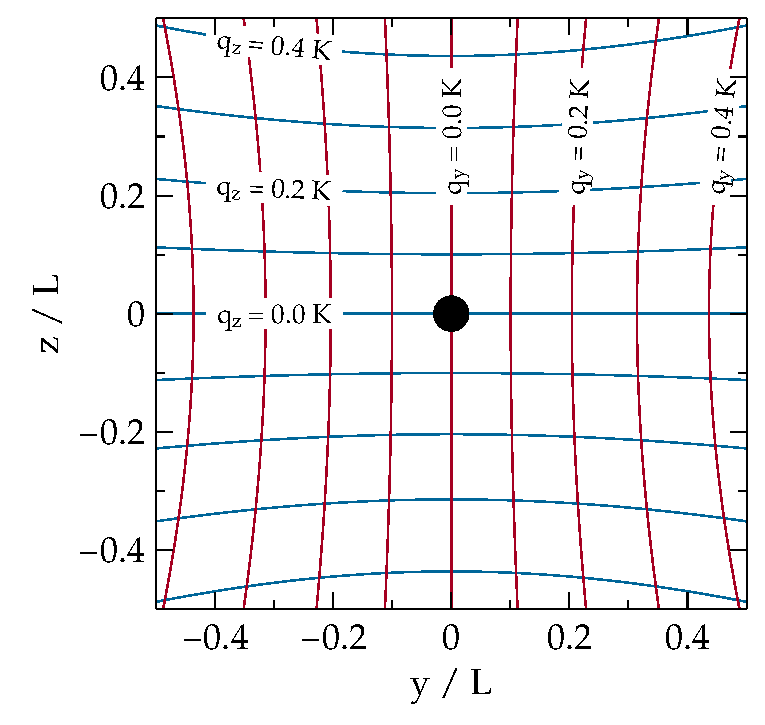
\includegraphics[width=.47\textwidth]{fig/drawing/SAS_const_q_yz.ps}
\end{center}
\caption{Lines of constant $q_x$ (left), $q_y$ or $q_z$ (right),
in units of the incident wavenumber $K=2\pi/\lambda$,
for a planar detector and a central incident beam as in Fig.~\protect\ref{Fconstalphi}.}
\label{Fconstq}
\end{figure}

The transform (\ref{Eqalgo}) between pixel coordinates $y$,~$z$
and physical scattering vector components $q_y$, $q_z$
is nonlinear, due to the square-root term in the denominator of~(\ref{Ekf_by_pixel}).
For $y,z\ll L$, however, nonlinear terms loose importance.
To emphasize nonlinearities,
Figs.~\ref{Fconstalphi}--\ref{Fconstp}
show the rather extreme conditions at scattering angles of up to 45$^\circ$,
which are unusually large angles by the standards of SAS or GISAS.
In most experimental situations,
angles, and therefore nonlinearities, are considerably smaller.

\begin{figure}[t]
\begin{center}
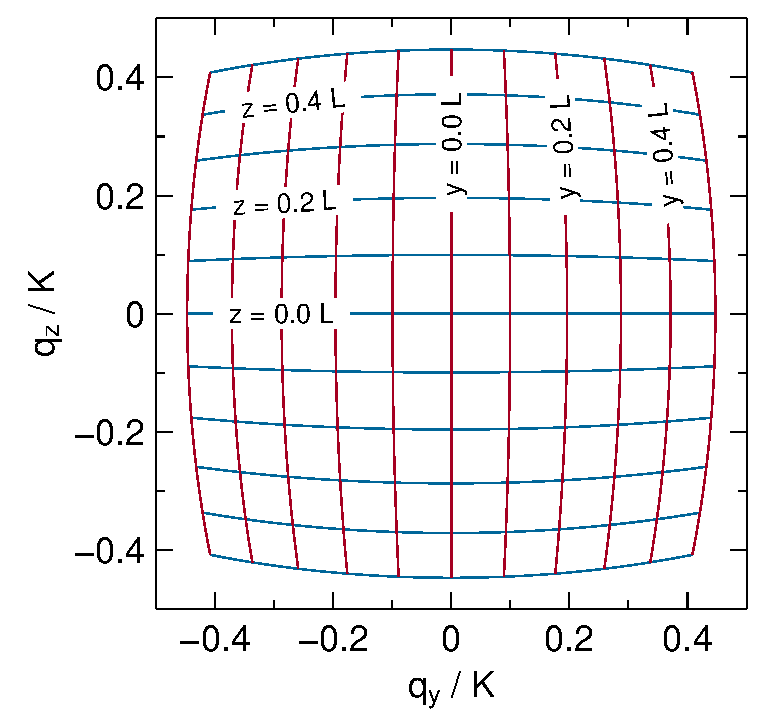
\includegraphics[width=.47\textwidth]{fig/drawing/SAS_const_p_yz.ps}
\end{center}
\caption{The outer contour of the blue and red grid
shows the border of a square detector image 
after transformation into the physical coordinates $q_y$,~$q_z$.
The blue and red curves correspond to horizontal and vertical lines in the detector.}
\label{Fconstp}
\end{figure}

The left detector frame in Fig.~\ref{Fconstq}
shows circles of constant values of $\pm q_x$.
For given steps in $q_x$, the distance between adjacent circles
increases towards the detector center.
From (\ref{Eq}) and (\ref{Ekf_by_pixel}),
one finds asymptotically for $y,z\to L$
that $q_x$ goes with the square of the two other components of the scattering vector,
\begin{equation}\label{Eqxasy}
  \frac{q_x}{K}
  \doteq \frac{y^2+z^2}{2 L^2} 
  \doteq \frac{q_y^2 + q_z^2}{2K^2}.
\end{equation}
Therefore, under typical small angle conditions $y,z\to L$
the dependence of the scattering signal on $q_x$ is unimportant:
one basically measures $\chi(\q)\simeq \chi(0,q_y,q_z)$.

\Work{Show consequences of $q_x$ for box example.}

As anticipated in (\ref{Eqxasy}),
the other two components of $\q$ are in first order linear in the pixel coordinates,
\begin{equation}
  \frac{q_y}{K}=\frac{y}{L}\left(1-\frac{y^2+z^2}{2L^2}+\ldots\right),
\end{equation}
and similarly for~$q_z$.
The nonlinear correction terms lead to the pincushion distortion 
shown in the right detector frame in Fig.~\ref{Fconstq}.
\index{Distortion!of $q_x$, $q_y$ grid in detector plane}%
\index{Detector!distortion of $q_x$, $q_y$ grid}%
\index{Pincushion distortion}%

Since pixel coordinates are meaningful only
with respect to a specific experimental setup,
users may wish to transform detector images
towards the physical coordinates $q_y$ and~$q_z$.
As shown in Fig.~\ref{Fconstp},
this would yield a barrel-shaped ilumminated area
in the $q_y$,~$q_z$~plane.

\Note{\indent Transforming detector images 
  from pixel coordinates into the $q_y$,~$q_z$~plane is not implemented in \BornAgain,
  and not on our agenda.
  We would, however, like to hear about use cases.}

\Emph{\indent When simulating and fitting experimental data with \BornAgain,
detector images remain unchanged.
All work is done in terms of reduced pixel coordinates $y/L$ and~$z/L$.
Corrections are applied to the simulated, not to the measured data.}

\Work{\indent \ldots show how to plot $q$ grid on top of detector image \ldots}

%Tradition wants that raw data be \E{treated} or \E{reduced}
%before they are \E{analyzed}.
%In our case, raw data reduction would comprise 
%the transform (\ref{Eqalgo}) of pixel coordinates into scattering vectors,
%and the accompanying renormalization (\ref{EItrafo}) of pixel counts.

%===============================================================================
\subsection{Symmetry}
%===============================================================================

\Work{to write ... and to continue in other chapters}

\index{Small-angle scattering|)}%
